\chapter{Introduction}

In this first chapter we want to introduce the reader to the topic to be covered in this thesis.
We will state the problem and explain the motivation for this work and the relevance it has in the field of agent oriented software development.
Finally we will describe how we attempt to solve it and give an outline of the following chapters.



\section{Motivation and Problem Description}

% agenten nächster größer schritt in software development
In the past years and decades multi-agent systems have evolved from science fiction to a promising field of research. In fact they could mark the next great leap in software architecture after imperative and object oriented programming by bringing the principles of reusability and modularity to a new level.

\begin{tabular}{p{5cm}|p{9cm}}
Imperative Programming &
        Programs can be subdivided into several functions.
\\\hline
Object Oriented Programming &
        Objects encapsulate data and functionality and can be shared between programs of the same language.
\\\hline
Multi-Agent Systems &
        Functionality is provided by agents and can be shared among programs of different languages. Services can be selected autonomously based on their precondition and effect.
\end{tabular}

% wenig beachtung in business welt, stattdessen nur webservices
Software agents and multi-agent systems have been researched for a long time now. But although they provide advanced concepts, some of which are now rediscovered by Service Oriented Architecture and web-services, they are still mainly an academic subject, while the uptake of agent technologies by the industry is very slow. Although they address the same problem, web-services have been adopted a lot faster and are by now well established in the business world.

% agenten zu komplex?
A reason for this could be the complexity of multi-agent system that might discourage business people and even experienced developers from giving agents a chance. The mentalistic notions used in agent technology seem to be too unfamiliar to the business people, who rather tend to think in terms of processes and web-services.

% unser approach
To bridge that gap that exists between the academic research and the industry and to facilitate the creation of multi-agent systems our approach is to allow agents to be designed and deployed using business process diagrams and thus to widen the clientèle of agent technology.


\subsection{Model Driven Engineering}
% model driven engineering
Following the principle of \emph{Model Driven Engineering} programs are no longer written, but specified in a number of models. These models are then used for generating the actual program code, facilitating and accelerating the software development process and resulting in high quality software. The modeler does not have to care too much about a language's details and the resulting programs are uniformly designed and thus easy to maintain and highly interoperable.

\begin{itemize}
	\item Usage of several models for different views on a system, for instance for control flow, data structures and distribution
	\item Independence of platform and programming language: One model can be used to generate the same programs for various languages and platforms.
	\item Automation of laborious tasks such as GUI building, exception handling and resource management
	\item Understandable, easily maintainable code
	\item Model validation
\end{itemize}

With the right metamodel and a mapping from that metamodel to agent concepts, Model Driven Engineering could be a great help when designing multi-agent systems.

% editor generation
Further, given today's model driven development tools, also feature-rich, visual editors for any domain can be designed and generated in a short time. Being created for designing business process models these editors then again can be used for the generation of executable programs based on these processes.


\subsection{Process Modeling and Business Process Diagrams}

% uml <-> process
Business Process Diagrams provide a very abstract view on a program. Although UML covers more aspects of software development and might be more popular among the developers, business process diagrams can quickly be drawn and are easily understandable for managers, business people and domain experts who are not always familiar with UML.

\begin{figure}[htp]
	\centering
	\includegraphics[width=.75\textwidth]{figures/examples/rss-client.png}
	\caption{Sample BPMN Diagram}
	\label{fig:bpmn_intro}
\end{figure}

% mini-intro bpmn
The Business Process Modeling Notation (BPMN) is a relatively new process modeling notation. As a standardized business process notation it is increasingly important. At the same time the clear and concise graphical notion, as seen in figure \ref{fig:bpmn_intro}, can be enriched with non-graphical elements and attributes and extended with artifacts, enabling a mapping to executable programming languages.

% unstructured workflows
However, the potential of mapping BPMN to executable languages suffers from the problem that BPMN diagrams can be arbitrary directed graphs while most programming languages are block structured, and thus BPMN has more expressive power than most programming languages. This issue has been discussed in many papers, often describing rule based approached for identifying block structures in BPMN diagrams or modifying unstructured diagrams.

% keine mappings nach agenten yet
But while the mapping from BPMN to BPEL, which is given in the specification, is implemented in a growing number of tools, there are to the author's best knowledge no implementations of a mapping from BPMN to multi-agent systems, yet.
\\

% agentensprachen pushen, business men können agenten benutzen. win-win.
A mapping from BPMN to agents, together with an easy-to-use tool implementing that mapping, will most likely increase the spreading of multi-agent systems and make the benefits of agent technology usable for business people.



\section{Goals}

Our goal is to develop a \textsc{Visual Service Design Tool} (fig. \ref{fig:vsdt}) that can be used for modeling business process diagrams and transforming these diagrams to executable JIAC programs. As a byproduct also a transformation to BPEL will be provided.

\begin{figure}[htp]
	\centering
	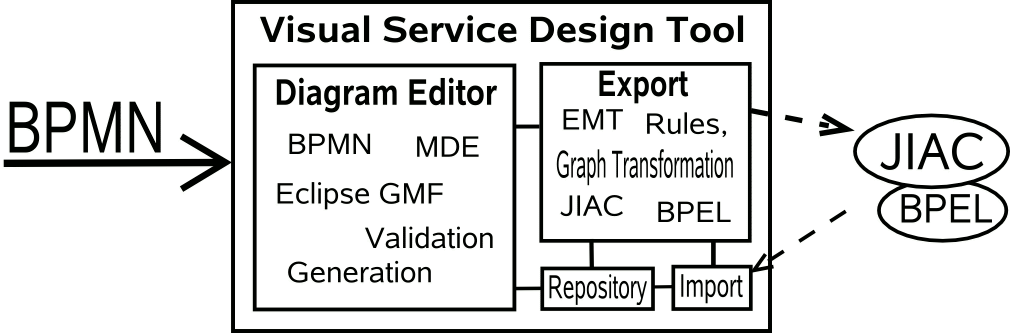
\includegraphics[width=.75\textwidth]{figures/intro.png}
	\caption{Our Vision of the Visual Service Design Tool}
	\label{fig:vsdt}
\end{figure}

The main challenges and requirements for achieving this are:
\begin{enumerate}

	\item The creation of the business process metamodel to be used for the process diagrams' internal representation. The model has to conform to a standardized business process notation so it can be intuitively understood by business people, but still has to be to some amount extensible. The model has to provide enough semantics to enable a mapping to executable languages, but still has to be easy to create and understand.
	
	\item The development of an easy to use, yet powerful editor for the creation of business process diagrams. Since the aim of this work is to facilitate the creation and to boost the distribution of multi-agent systems the editor has to be easy to use so it can be operated by non-experts, business users and domain experts, too. It has to provide the usual editing features and a way to validate the diagrams to conform to the underlying specification.
	
	\item The development of a mapping from BPMN to JIAC IV. While most elements of BPMN map nicely to various JADL statements the original BPMN notation lacks an equivalent to JIAC Agents, thus we will have to discuss whether one of the existing BPMN elements can be used for this or whether the specification will need to be extended by additional elements for this purpose.
	
	\item The implementation of that mapping as a transformation tool. The export features have to be extensible and usable together with the editor. The structural differences between BPMN diagrams and BPEL and JIAC programs will require a number of rules for identifying and transforming block structured in BPMN diagrams.

\end{enumerate}

With this tool the user can draw a high-level BPMN process diagram and generate code from it. Depending on the level of detail of the process model the resulting program will still need some refinement, but given a very detailed model the program could be executable right after its creation.



\section{Outline}

% jiac und pml
In chapter \ref{chapter:processes} we will introduce the reader to the agent description language JADL and the JIAC framework and give an overview on existing process modeling languages that might be adequate for modeling agent systems. We will explain why we decided for BPMN and list its most important features.

% mde
In chapter \ref{chapter:mde} we will give a short introduction to Model Driven Engineering and have a look on EMF and GMF. Further we will discuss the model driven development of processes, especially when based on unstructured process models, and list some existing approaches in transforming business process diagrams to executable BPEL processes and agent systems.

% trafo tools
After that, chapter \ref{chapter:transformation} will introduce the rule-based transformation framework being used in this work.

In chapter \ref{chapter:jiacMapping} the mappings from BPMN to BPEL and JIAC will be explained in detail.

% implementation: editor, mapping
In chapter \ref{chapter:impl_editor} we will review the development of the \textsc{Visual Service Design Tool} and in chapter \ref{chapter:impl_mapping} we will describe the transformation modules used for the mapping from BPMN to BPEL and JIAC. We will outline the concept, have a look on the several stages of the mapping and introduce the most important rules. Chapter \ref{chapter:examples} will give some examples of the transformation from BPMN to JIAC.

% conclusion
Finally, chapter \ref{chapter:conclusion} will give the conclusion of this thesis and state some ideas and topics for future work to be done on this topic.

% appendix: user manual
In the appendix of this work the reader can find a user manual for the diagram editor.